%* --- Options for printing (twoside) or digital (oneside) --- %
\newif\ifPRINTING
%\PRINTINGtrue %! Set the conditional to true
\PRINTINGfalse %! Set the conditional to false (one must be commented out)

\ifPRINTING
    \documentclass[british, twoside]{ntnuthesis}  % Language options: british, american, norsk, nynorsk
\else
    \documentclass[british, oneside]{ntnuthesis}  % Language options: british, american, norsk, nynorsk
\fi


%* --- Import of additional preamble files (advanced) --- %
\usepackage{import}  % import package allows for loading self-made .sty files
\usepackage{preamble/head_mk2}


%* --- Import support files --- %

%* Author
\author{Hauge, Max}
\shortauthor{MH}


%* Supervisor(s)
\newif\ifSINGLESUPERVISOR
%\SINGLESUPERVISORtrue  %! Set the conditional to true
\SINGLESUPERVISORfalse  %! Set the conditional to false

\ifSINGLESUPERVISOR
    \newcommand{\supervisorGrammar}{Supervisor}
    \newcommand{\supervisor_A}{Grepstad, Sigrid}
\else
    \newcommand{\supervisorGrammar}{Supervisors}
    \newcommand{\supervisorA}{Grepstad, Sigrid}
    \newcommand{\supervisorB}{Heap, Winston}  % For more supervisors add a new line here and update the temporary title-page 'titlepage_max.tex' file
\fi


%* Title
\title{Plaser Din Fancy Lange Tittel Her}
\shorttitle{Master's thesis}


%* Course name / Emnekode
\newcommand{\emnekode}{MA3911 — masteroppgave i matematiske fag}


%* Institutt
%? The command is the same no matter the language: bokmål, nynorsk, british, american
%? If changing between languages many times either update the "ntnuthesis.cls" file directly and comment out the code here
%? Or simply comment in/out the used/unused commands manually here each time you change the language
\renewcommand{\NTNUinstitutt}{Institute of Mathematical Sciences}
\renewcommand{\NTNUinstituttLowerC}{institute of mathematical sciences}


%* Date
\date{\today}
  %! Remember to update the content here
%
% From https://www.overleaf.com/learn/latex/Glossaries

\makeglossaries % Prepare for adding glossary entries


\newglossaryentry{latex}
{
        name=latex,
        description={Is a mark up language specially suited for
scientific documents}
}

\newglossaryentry{bibliography}
{
        name=bibliography,
        plural=bibliographies,
        description={A list of the books referred to in a scholarly work,
typically printed as an appendix}
}

\newglossaryentry{maths}
{
    name=mathematics,
    description={Mathematics is what mathematicians do}
}


% --------------------
% ----- Acronyms -----
% --------------------

\newacronym{phd}{PhD}{philosophiae doctor}
\newacronym{CoPCSE}{CoPCSE@NTNU}{Community of Practice in Computer ScienceEducation at NTNU}
\newacronym{gcd}{GCD}{Greatest Common Divisor}
  % add glossary and acronym lists before document. Add \printglossaries after \tableofcontents to print

%% Commands for the document
%% ---------------------------------------------------------------------

% Defines a new command for the horizontal lines, change thickness here
\newcommand{\HRule}{\rule{\linewidth}{0.5mm}} 
%\renewcommand{\arraystretch}{1.25}



%% Mathematical symbol commands
%% ---------------------------------------------------------------------
%\newcommand{\N}{\mathbb{N}}  % Already defined
\newcommand{\Z}{\mathbb{Z}}
\newcommand{\bbP}{\mathbb{P}}
\newcommand{\PP}{\mathbb{PP}}
\newcommand{\Q}{\mathbb{Q}}
\newcommand{\R}{\mathbb{R}}
%\newcommand{\C}{\mathbb{C}}  % Already defined
\newcommand{\Fp}{\mathbb{F}_p}
\newcommand{\Fq}{\mathbb{F}_q}


\newcommand{\Tau}{\mathrm{T}}

%% Z med striketrhough
\newcommand{\Zstroke}{\text{\ooalign{\hidewidth\raisebox{0.2ex}{--}\hidewidth\cr$Z$\cr}}}
\newcommand{\zstroke}{\text{\ooalign{\hidewidth -\kern-.3em-\hidewidth\cr$z$\cr}}}



\newcommand{\degc}{$^\circ$C~}
\renewcommand{\deg}{\ensuremath{^{\circ}}}
\newcommand{\edegc}{^\circ \text{C}~}
\newcommand{\minone}{$^{-1}$}
\newcommand{\eminone}{^{-1}}



%% Other Settings
%% ---------------------------------------------------------------------
% \masl{m.a.s.l}


% --- Macros --- %
% User defined macros (functions) can go here, 
% these may be overriden for each subfile by using \renewcommand{}[][]{}
\newcommand{\set}[1]{\{#1\}} % A macro for making a set

%% normal-brackets
\newcommand{\brac}[1]{\left(#1\right)}
%% Square-brackets
\newcommand{\bras}[1]{\left[#1\right]}
%% Curly-brackets
\newcommand{\braq}[1]{\left\{#1\right\}}


\newcommand{\spn}[1]{\operatorname{span}\left( #1 \right)}
\newcommand{\spnclos}[1]{\overline{\operatorname{span}}\left( #1 \right)}
\newcommand{\mes}[1]{\operatorname{mes}\left( #1 \right)}  % add commands before document
\addbibresource{support_files/Mastergrad.bib}  % add the Bibliography file

%! Two-side option
%! Must manually check whether the page offset appears correctly on each 'left' and 'right' page. 
%? If the code is commented out (i.e. the offset appears on the wrong pages), then one also needs to update the headers in 'ntnuthesis.cls'
\ifPRINTING
    % The following code "flips" the offset for the 'left' and 'right' pages
    \let\tmp\oddsidemargin
    \let\oddsidemargin\evensidemargin
    \let\evensidemargin\tmp
    \reversemarginpar
\fi

%* —————————————  THE DOCUMENT  ————————————— %
\begin{document}
    %* --- Opening --- %
    %? Remember to comment out the title page when creating the final front page required by NTNU
    % Title for the document
% --------------------------------------------------------------------------

\begin{titlepage}
	\makeatletter
	\let\thetitle\@title
	\let\theauthor\@author
	\let\thedate\@date
	\makeatother

	\centering
    \vspace*{0.5 cm}
    % University Logo
    
\includegraphics[width=0.7\textwidth]{ntnu.png}\\[1.0 cm]
    
	% University Name
	\textsc{\LARGE \textsf{\NTNULowerC}}\\[1.0 cm]  %* sans serif no caps
	%\textsc{\LARGE \textsf{\NTNU}}\\[1.0 cm]  %* sans serif caps
    %\textsc{\LARGE \NTNU}\\[1.0 cm]  %* RM caps
    
	% Institute
	\textsc{\Large \textsf{\NTNUinstituttLowerC}}\\[0.5 cm]  %* sans serif no caps
    %\textsc{\Large \NTNUinstitutt}\\[0.5 cm]  %* RM caps
	
	% Course Name
	\textsc{\large \textsf{\emnekode}}\\[0.5 cm]  %* sans serif no caps
	%\textsc{\large \emnekode}\\[0.5 cm]  %* RM caps
	
	%------------
	\rule{\linewidth}{0.2 mm} \\[0.4 cm]
	{ \LARGE \textbf{\textsf{\uppercase{\thetitle}}}}\\
	\rule{\linewidth}{0.2 mm} \\[1.0 cm]%[1.5 cm]
	
	

%! When the figure is used in the title, the figure environment is removed

%\begin{figure*}[h!]
%    \centering
    %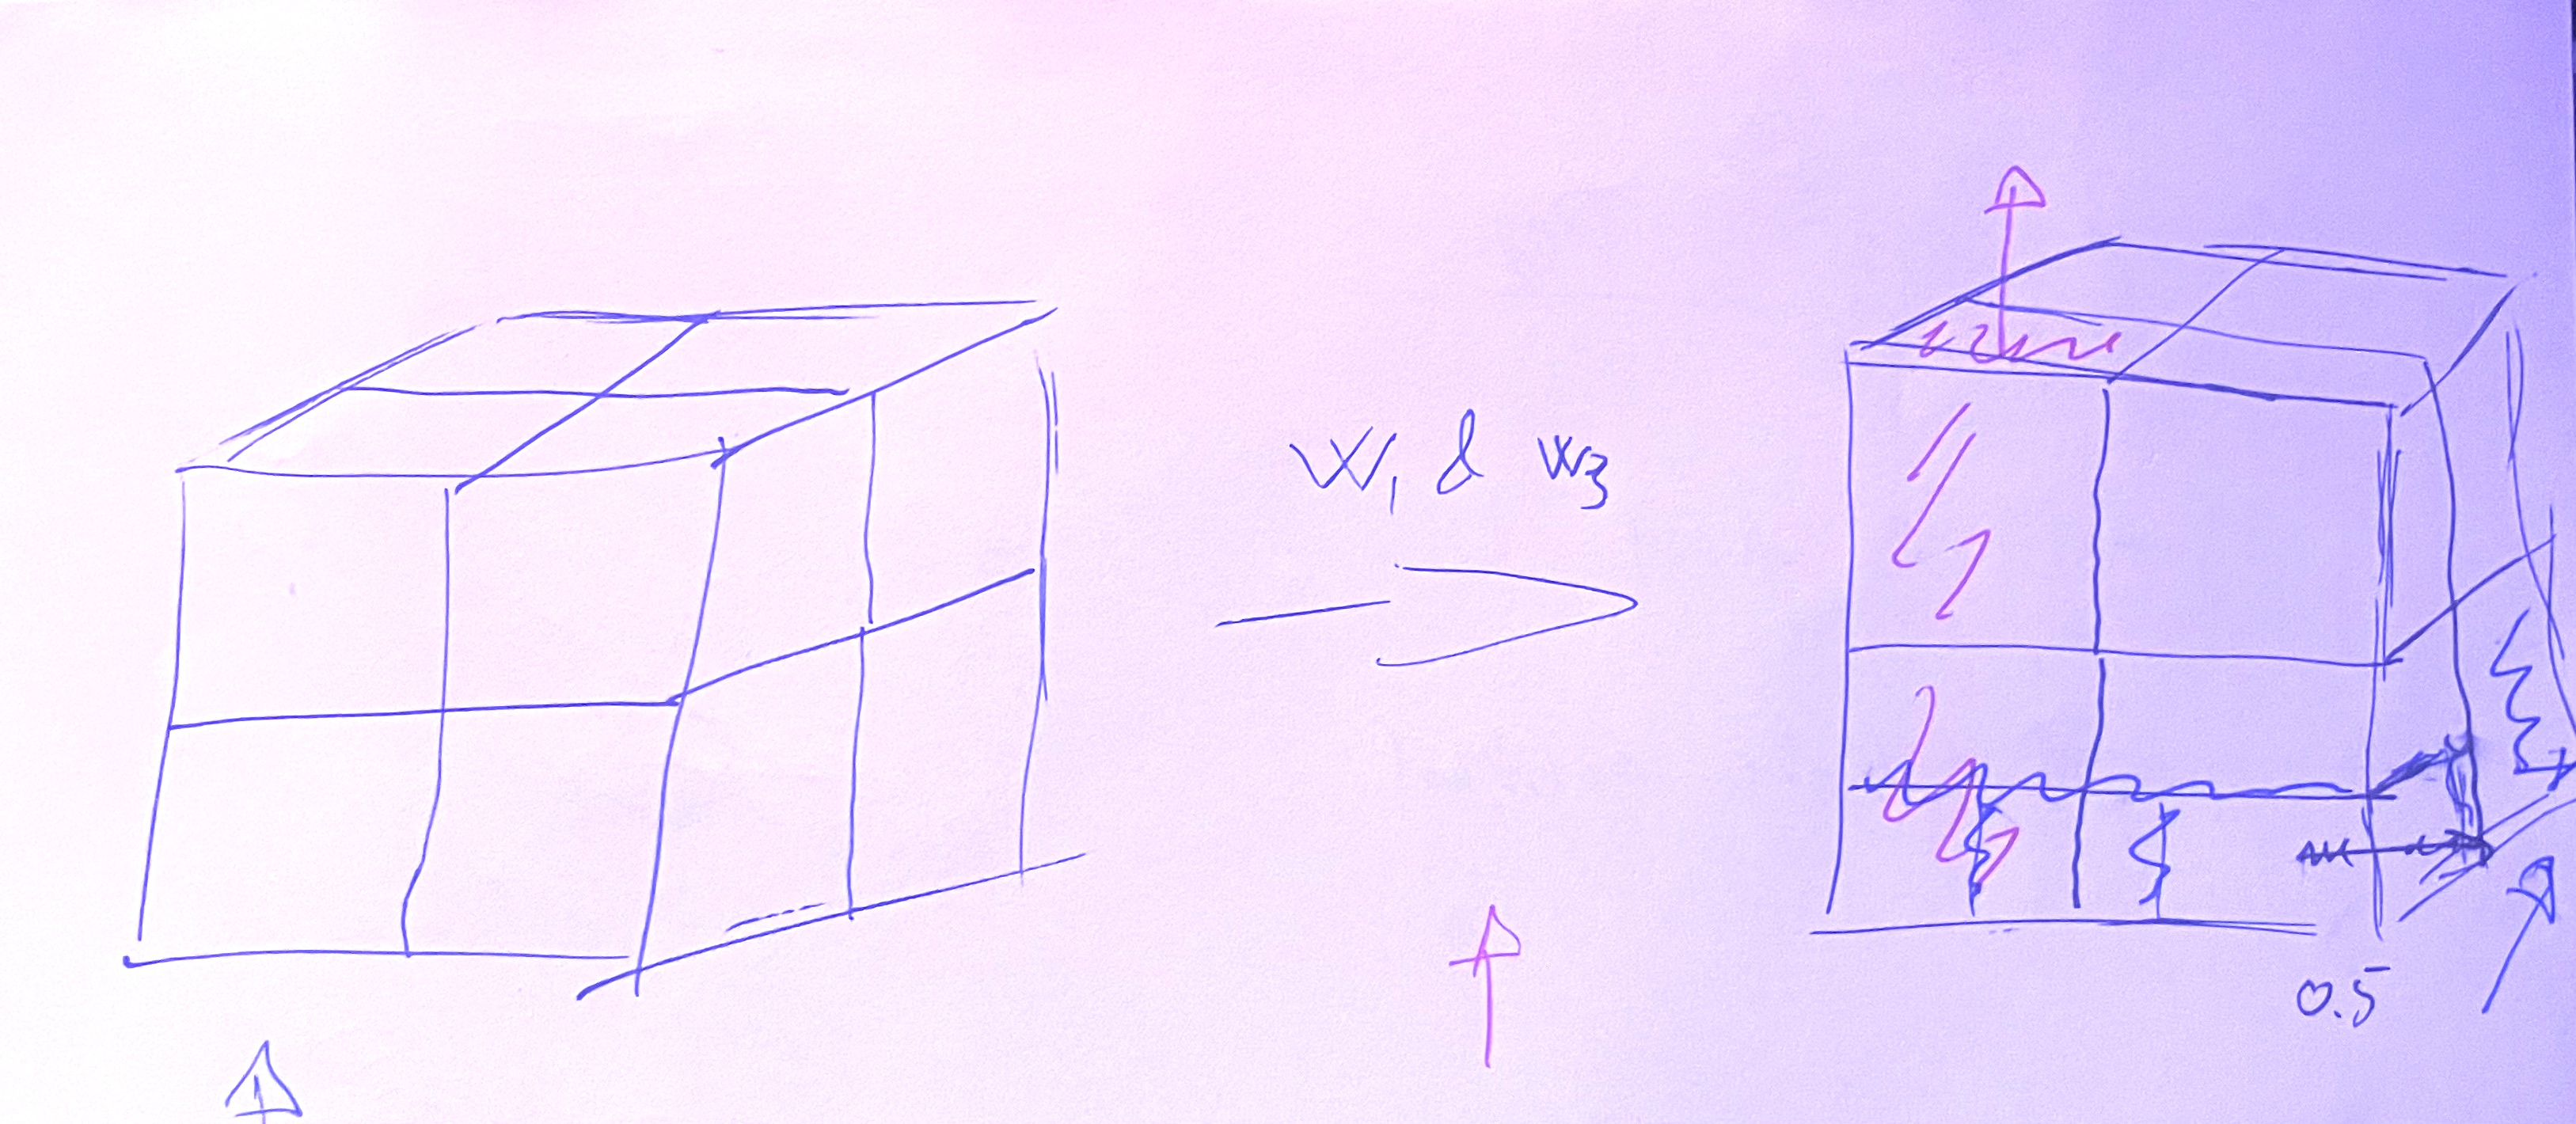
\includegraphics[width=0.87\linewidth]{aper_yeye.jpg}
    %* Figure
    % for the use in the online editor: \usepackage{tikz} 
    \begin{tikzpicture}[scale=0.9] %! The original scale is 1
        % Define the tile
        \def\tile{
        % Draw the unit cube
            \draw[black!95] (1,0,0) -- (1,0,1) -- (1,1,1) -- (1,1,0) -- cycle; % left face
            \draw[black!95] (0,0,0) -- (1,0,0) -- (1,0,1) -- (0,0,1) -- cycle; % bottom face
            \draw[black!95] (0,0,0) -- (0,1,0) -- (1,1,0) -- (1,0,0) -- cycle; % back face
            \draw[black!95, fill=gray!65] (1,0,0) -- (1,1,0) -- (1,1,1) -- (1,0,1) -- cycle; % right face
            \draw[black!95, fill=white] (0,0,1) -- (1,0,1) -- (1,1,1) -- (0,1,1) -- cycle; % front face
            \draw[black!95, fill=white](0,1,0) -- (0,1,1) -- (1,1,1) -- (1,1,0) -- cycle; % top face
        }

        \def\tilecolumn{
            % Draw the unit cube
                \draw[black!95] (1,0,0) -- (1,0,1) -- (1,1,1) -- (1,1,0) -- cycle; % left face
                \draw[black!95] (0,0,0) -- (1,0,0) -- (1,0,1) -- (0,0,1) -- cycle; % bottom face
                \draw[black!95] (0,0,0) -- (0,1,0) -- (1,1,0) -- (1,0,0) -- cycle; % back face
                \draw[black!95, fill=cyan] (1,0,0) -- (1,1,0) -- (1,1,1) -- (1,0,1) -- cycle; % right face
                \draw[black!95, fill=cyan] (0,0,1) -- (1,0,1) -- (1,1,1) -- (0,1,1) -- cycle; % front face
                \draw[black!95, fill=cyan](0,1,0) -- (0,1,1) -- (1,1,1) -- (1,1,0) -- cycle; % top face
            }
        
        \def\tilerow{
            % Draw the unit cube
                \draw[black!95] (1,0,0) -- (1,0,1) -- (1,1,1) -- (1,1,0) -- cycle; % left face
                \draw[black!95] (0,0,0) -- (1,0,0) -- (1,0,1) -- (0,0,1) -- cycle; % bottom face
                \draw[black!95] (0,0,0) -- (0,1,0) -- (1,1,0) -- (1,0,0) -- cycle; % back face
                \draw[black!95, fill=orange] (1,0,0) -- (1,1,0) -- (1,1,1) -- (1,0,1) -- cycle; % right face
                \draw[black!95, fill=orange] (0,0,1) -- (1,0,1) -- (1,1,1) -- (0,1,1) -- cycle; % front face
                \draw[black!95, fill=orange](0,1,0) -- (0,1,1) -- (1,1,1) -- (1,1,0) -- cycle; % top face
            }
    
        % Draw the tiling pattern LEFT: x = 0,1,2,3
        % not shifted
        % the backseat boys
        \foreach \x in {0,1,2,3}{
            \foreach \y in {-2,-1,0,1}{
                \foreach \z in {-2,-1}{
                    \pgfmathsetmacro{\shiftX}{\x}
                    \pgfmathsetmacro{\shiftY}{\y}
                    \pgfmathsetmacro{\shiftZ}{\z}
                    
                    \begin{scope}[shift={(\shiftX,\shiftY,\shiftZ)}]
                    \tile % Draw the tile
                    \end{scope}
                }
            }
        }
        % Draw the back four cubes as two rows for the shift in X
        % not shifted
        \foreach \x in {0,1,2,3}{
            \foreach \y in {-2,-1,0}{
                \foreach \z in {0}{
                    \pgfmathsetmacro{\shiftX}{\x}
                    \pgfmathsetmacro{\shiftY}{\y}
                    \pgfmathsetmacro{\shiftZ}{\z}
                    
                    \begin{scope}[shift={(\shiftX,\shiftY,\shiftZ)}]
                    \tile % Draw the tile
                    \end{scope}
                }
            }
        }
        % Will be shifted – in the X direction
        \foreach \x in {0,1,2,3}{
            \foreach \y in {1}{
                \foreach \z in {0}{
                    \pgfmathsetmacro{\shiftX}{\x}
                    \pgfmathsetmacro{\shiftY}{\y}
                    \pgfmathsetmacro{\shiftZ}{\z}
                    
                    \begin{scope}[shift={(\shiftX,\shiftY,\shiftZ)}]
                    \tilerow % Draw the tile
                    \end{scope}
                }
            }
        }
        
        
        % not shifted
        \foreach \x in {0}{
            \foreach \y in {-2,-1,0,1}{
                \foreach \z in {1}{
                    \pgfmathsetmacro{\shiftX}{\x}
                    \pgfmathsetmacro{\shiftY}{\y}
                    \pgfmathsetmacro{\shiftZ}{\z}
                    
                    \begin{scope}[shift={(\shiftX,\shiftY,\shiftZ)}]
                    \tile % Draw the tile
                    \end{scope}
                }
            }
        }
        % Draw the front four cubes as two columns for the shift in Y
        % Will be shifted – in the Y direction
        \foreach \x in {1}{
            \foreach \y in {-2,-1,0,1}{
                \foreach \z in {1}{
                    \pgfmathsetmacro{\shiftX}{\x}
                    \pgfmathsetmacro{\shiftY}{\y}
                    \pgfmathsetmacro{\shiftZ}{\z}
                    
                    \begin{scope}[shift={(\shiftX,\shiftY,\shiftZ)}]
                    \tilecolumn % Draw the tile
                    \end{scope}
                }
            }
        }
        % not shifted
        \foreach \x in {2,3}{
            \foreach \y in {-2,-1,0,1}{
                \foreach \z in {1}{
                    \pgfmathsetmacro{\shiftX}{\x}
                    \pgfmathsetmacro{\shiftY}{\y}
                    \pgfmathsetmacro{\shiftZ}{\z}
                    
                    \begin{scope}[shift={(\shiftX,\shiftY,\shiftZ)}]
                    \tile % Draw the tile
                    \end{scope}
                }
            }
        }
        
        % Draw the Inbetween stuff
        %———————————————————————————————————
        \draw[->, thick, black] (5.5,0.2) -- (7.5,0.2);
        \node[black] at (6.6,0.5) {\Large $\upsilon',\upsilon''$}; 
        
        
        
        
        % Draw the tiling pattern RIGHT: x= 9,10,11,12
        %———————————————————————————————————
        % not shifted
        % the backseat boys
        \foreach \x in {9,10,11,12}{
            \foreach \y in {-2,-1,0,1}{
                \foreach \z in {-2,-1}{
                    \pgfmathsetmacro{\shiftX}{\x}
                    \pgfmathsetmacro{\shiftY}{\y}
                    \pgfmathsetmacro{\shiftZ}{\z}
                    
                    \begin{scope}[shift={(\shiftX,\shiftY,\shiftZ)}]
                    \tile % Draw the tile
                    \end{scope}
                }
            }
        }
        % Draw the back four cubes as two rows for the shift in X
        % not shifted
        \foreach \x in {9,10,11,12}{
            \foreach \y in {-2,-1,0}{
                \foreach \z in {0}{
                    \pgfmathsetmacro{\shiftX}{\x}
                    \pgfmathsetmacro{\shiftY}{\y}
                    \pgfmathsetmacro{\shiftZ}{\z}
                    
                    \begin{scope}[shift={(\shiftX,\shiftY,\shiftZ)}]
                    \tile % Draw the tile
                    \end{scope}
                }
            }
        }
        % Will be shifted – in the X direction
        \foreach \x in {8,9,10,11,12}{
            \foreach \y in {1}{
                \foreach \z in {0}{
                    \pgfmathsetmacro{\shiftX}{\x+0.5}
                    \pgfmathsetmacro{\shiftY}{\y}
                    \pgfmathsetmacro{\shiftZ}{\z}
                    
                    \begin{scope}[shift={(\shiftX,\shiftY,\shiftZ)}]
                    \tilerow % Draw the tile
                    \end{scope}
                    
                    %\ifnum\x=9
                    %    \draw[->, orange] (\shiftX+1,1.4) --node[below] {$0.5$} (\shiftX+2,1.4);             \fi
                }
            }
        }
        

        % not shifted
        \foreach \x in {9}{
            \foreach \y in {-2,-1,0,1}{
                \foreach \z in {1}{
                    \pgfmathsetmacro{\shiftX}{\x}
                    \pgfmathsetmacro{\shiftY}{\y}
                    \pgfmathsetmacro{\shiftZ}{\z}
                    
                    \begin{scope}[shift={(\shiftX,\shiftY,\shiftZ)}]
                    \tile % Draw the tile
                    \end{scope}
                }
            }
        }
        % Draw the front four cubes as two columns for the shift in Y
        % Will be shifted – in the Y direction
        \foreach \x in {10}{
            \foreach \y in {-3,-2,-1,0,1}{
                \foreach \z in {1}{
                    \pgfmathsetmacro{\shiftX}{\x}
                    \pgfmathsetmacro{\shiftY}{\y+0.5}
                    \pgfmathsetmacro{\shiftZ}{\z}
                    
                    \begin{scope}[shift={(\shiftX,\shiftY,\shiftZ)}]
                    \tilecolumn % Draw the tile
                    \end{scope}
                    
                    %\ifnum\y=1
                    %    \draw[->, thick, cyan] (7,\shiftY+0.5) --node[right] {$0.5$} (7,\shiftY+1.5);             \fi
                }
            }
        }
        % not shifted
        \foreach \x in {11,12}{
            \foreach \y in {-2,-1,0,1}{
                \foreach \z in {1}{
                    \pgfmathsetmacro{\shiftX}{\x}
                    \pgfmathsetmacro{\shiftY}{\y}
                    \pgfmathsetmacro{\shiftZ}{\z}
                    
                    \begin{scope}[shift={(\shiftX,\shiftY,\shiftZ)}]
                    \tile % Draw the tile
                    \end{scope}
                }
            }
        }
        
        
  
    \end{tikzpicture}
    %\caption{Illisustrated in the \cref{fig:big_aperi} is simply a bigger version of the aperiodic tile we have constructed.}
    %\label{fig:big_aperi}
%\end{figure*}


	% Page setup
	\begin{minipage}{0.4\textwidth}
		\begin{flushleft} \large
			\emph{Author:}\\
			\textrm{\theauthor}
		\end{flushleft}
	\end{minipage}
	\begin{minipage}{0.4\textwidth}
		\begin{flushright} \large
			\emph{\supervisorGrammar:} \\
			\textrm{\supervisorA}\\  % Supervisor #1
			\textrm{\supervisorB} %\\  % Supervisor #2
			%\textrm{ } %\\  % Supervisor #3
		\end{flushright}
	\end{minipage}\\[1.5 cm]
	

	{\large \thedate}%\\[2 cm]
 
	%\vfill

\end{titlepage}

  %! Temporary title page for your project
    
%? Note: We have "Clearpage" automatically after the title page

%* Abstract
\thispagestyle{plain}




%\thispagestyle{plain}

\begin{center}\textsf{\textbf{\large Abstract}}\end{center} 

Lorem ipsum dolor sit amet, consectetur adipiscing elit, sed do eiusmod tempor incididunt ut labore et dolore magna aliqua.

\begin{center}\textsf{\textbf{\large Sammendrag}}\end{center} 

Lorem ipsum dolor sit amet, consectetur adipiscing elit, sed do eiusmod tempor incididunt ut labore et dolore magna aliqua.


 
\addcontentsline{toc}{chapter}{Abstract}
\clearpage


%* Preface & acknowledgements
\ifPRINTING
    % This puts the quote on the "left double page with the Preface on the right"
    
% Adjust margins if needed
\ifPRINTING
    \newgeometry{top=0.5in, bottom=0.5in, left=1in, right=1in, bindingoffset=6mm}
\else
    \newgeometry{top=0.5in, bottom=0.5in, left=1in, right=1in}
\fi


\thispagestyle{empty} % Remove page number


\vspace*{\fill}
\begin{center}
    \textit{\enquote{A famous person once said...}}\\
\end{center}
\begin{flushright}
    \textbf{— Max in writing this document}
\end{flushright}
\vspace*{\fill}

\restoregeometry % Restore original page margins

    \chapter*{Preface}
    


\vspace{.25in}

Lorem ipsum dolor sit amet, consectetur adipiscing elit, sed do eiusmod tempor incididunt ut labore et dolore magna aliqua. Ut enim ad minim veniam, quis nostrud exercitation ullamco laboris nisi ut aliquip ex ea commodo consequat.

Lorem ipsum dolor sit amet, \textsc{Navn Navnesen}, consectetur adipiscing elit, sed do eiusmod tempor incididunt ut labore et dolore magna aliqua. Ut enim ad minim veniam, quis nostrud exercitation ullamco laboris nisi ut aliquip ex ea commodo consequat. Duis aute irure dolor in reprehenderit in voluptate velit esse cillum dolore eu fugiat nulla pariatur. Excepteur sint occaecat cupidatat non proident, \textsc{Navn Navnesen}, sunt in culpa qui officia deserunt mollit anim id est laborum.

Lorem ipsum dolor sit amet, consectetur adipiscing elit, sed do eiusmod tempor incididunt ut labore et dolore magna aliqua. Ut enim ad minim veniam, quis nostrud exercitation ullamco laboris nisi ut aliquip ex ea commodo consequat. Duis aute irure dolor in reprehenderit in voluptate velit esse cillum dolore eu fugiat nulla pariatur. Excepteur sint occaecat cupidatat non proident, sunt in culpa qui officia deserunt mollit anim id est laborum.

Lorem ipsum dolor sit amet, consectetur adipiscing elit, sed do eiusmod tempor incididunt ut labore et dolore magna aliqua. Ut enim ad minim veniam, quis nostrud exercitation ullamco laboris nisi ut aliquip ex ea commodo consequat. Duis aute irure dolor in reprehenderit in voluptate velit esse cillum dolore eu fugiat nulla pariatur. Excepteur sint occaecat cupidatat non proident, sunt in culpa qui officia deserunt mollit anim id est laborum.

\vspace*{1cm}

\begin{flushright}
    Max Lunde Hauge\\
    Trondheim, June 2023
\end{flushright}

\else
    % This puts the quote on the page after the Preface
    \chapter*{Preface}
    


\vspace{.25in}

Lorem ipsum dolor sit amet, consectetur adipiscing elit, sed do eiusmod tempor incididunt ut labore et dolore magna aliqua. Ut enim ad minim veniam, quis nostrud exercitation ullamco laboris nisi ut aliquip ex ea commodo consequat.

Lorem ipsum dolor sit amet, \textsc{Navn Navnesen}, consectetur adipiscing elit, sed do eiusmod tempor incididunt ut labore et dolore magna aliqua. Ut enim ad minim veniam, quis nostrud exercitation ullamco laboris nisi ut aliquip ex ea commodo consequat. Duis aute irure dolor in reprehenderit in voluptate velit esse cillum dolore eu fugiat nulla pariatur. Excepteur sint occaecat cupidatat non proident, \textsc{Navn Navnesen}, sunt in culpa qui officia deserunt mollit anim id est laborum.

Lorem ipsum dolor sit amet, consectetur adipiscing elit, sed do eiusmod tempor incididunt ut labore et dolore magna aliqua. Ut enim ad minim veniam, quis nostrud exercitation ullamco laboris nisi ut aliquip ex ea commodo consequat. Duis aute irure dolor in reprehenderit in voluptate velit esse cillum dolore eu fugiat nulla pariatur. Excepteur sint occaecat cupidatat non proident, sunt in culpa qui officia deserunt mollit anim id est laborum.

Lorem ipsum dolor sit amet, consectetur adipiscing elit, sed do eiusmod tempor incididunt ut labore et dolore magna aliqua. Ut enim ad minim veniam, quis nostrud exercitation ullamco laboris nisi ut aliquip ex ea commodo consequat. Duis aute irure dolor in reprehenderit in voluptate velit esse cillum dolore eu fugiat nulla pariatur. Excepteur sint occaecat cupidatat non proident, sunt in culpa qui officia deserunt mollit anim id est laborum.

\vspace*{1cm}

\begin{flushright}
    Max Lunde Hauge\\
    Trondheim, June 2023
\end{flushright}

    
% Adjust margins if needed
\ifPRINTING
    \newgeometry{top=0.5in, bottom=0.5in, left=1in, right=1in, bindingoffset=6mm}
\else
    \newgeometry{top=0.5in, bottom=0.5in, left=1in, right=1in}
\fi


\thispagestyle{empty} % Remove page number


\vspace*{\fill}
\begin{center}
    \textit{\enquote{A famous person once said...}}\\
\end{center}
\begin{flushright}
    \textbf{— Max in writing this document}
\end{flushright}
\vspace*{\fill}

\restoregeometry % Restore original page margins

\fi


%* Table of contents
\setcounter{tocdepth}{2}
\tableofcontents

%! Two-side option
%! Must manually check whether this is needed depending on length of 'toc'
% Blank page to avoid having Chapter 1 and 'toc' on the same "double page"
\ifPRINTING
    \newpage
    \thispagestyle{empty}
    \vspace*{\fill}
    \clearpage
\fi



    %* --- DOCUMENT START --- %
    %? --- NOTE: Folder structure --- %
    % 1. Allows compilation of each subfile rather than compiling everything at once each time
    % 2. Subfiles must have this file as an option while using the "documentclass" subfile
    % 3. Loading a subfile is done with \subfile{"path-to-file"}
    % 4. Remember to use the template to get all the right \subfile commands in each .tex document
    % ---
    
    % Chapter 1
    \chapter{Introduction}
        \subfile{chapters/01_introduction.tex}
    
    % Chapter 2
    \chapter{LaTeX Documents Hacks}
        \subfile{chapters/02_preliminaries.tex}
    
    % Chapter 3
    \chapter{TiPs}\label{chap:tiling}
        \subfile{chapters/03_writing_tips.tex}

    % Bibliography
    \printbibliography

    %! Two-side option
    %! Must manually check whether the last page of the bibliography ends on the "left" or "right" side of the "double page".
    %! The back cover from NTNU should be "alone" when using the "two-page" view mode in the PDF reader. 
    \ifPRINTING
    \newpage
    \thispagestyle{empty}
    \vspace*{\fill}
    \clearpage
    \fi
\end{document}
